\documentclass[10pt,UTF8]{ctexart}


\usepackage[margin=2cm,a4paper]{geometry}
%\usepackage[left=0.75in,top=0.6in,right=0.75in,bottom=1.0in,a4paper]{geometry}

\setmainfont{Caladea}
%% 也可以選用其它字庫:
% \setCJKmainfont[%
%   ItalicFont=AR PL KaitiM GB,
%   BoldFont=Noto Sans CJK SC,
% ]{Noto Serif CJK SC}
% \setCJKsansfont{Noto Sans CJK SC}
% \renewcommand{\kaishu}{\CJKfontspec{AR PL KaitiM GB}}

% 繁體中文
\setCJKmainfont[Path=fonts/ ]{NotoSansTC-Medium.otf}

\usepackage{minted}
\usepackage[breaklinks]{hyperref}

% Picture
% 導言區的此三行無變化
\usepackage{graphicx}
\usepackage{float} 
\usepackage{subfigure}
% 以下是新增的自定義格式更改
\usepackage[]{caption2} %新增調用的宏包
\renewcommand{\figurename}{Fig.} %重定義編號前綴詞
\renewcommand{\captionlabeldelim}{.~} %重定義分隔符
 %\roman 是羅馬數字編號,\alph是默認的字母編號,\arabic是阿拉伯數字編號,可按需替換下一行的相應位置
\renewcommand{\thesubfigure}{(\roman{subfigure})}%此外,還可設置圖編號顯示格式,加括號或者不加括號
\makeatletter \renewcommand{\@thesubfigure}{\thesubfigure \space}%子圖編號與名稱的間隔設置
\renewcommand{\p@subfigure}{} \makeatother

% Math
\usepackage {mathtools}
\usepackage{amssymb}

% Code
\usepackage{listings}
\usepackage{xcolor}
\lstset{
    % backgroundcolor=\color{red!50!green!50!blue!50},
    % 程式碼塊背景色為淺灰色
    rulesepcolor= \color{gray}, % 程式碼塊邊框顏色
    breaklines=true,  % 程式碼過長則換行
    numbers=left, % 行號在左側顯示
    numberstyle= \small,% 行號字型
    % eywordstyle= \color{red,% 關鍵字顏色
    commentstyle=\color{gray}, % 註釋顏色
    frame=shadowbox % 用方框框住程式碼塊
    }

\usepackage{hyperref}

\usepackage{multicol} %用于实现在同一页中实现不同的分栏

\title{人工智慧作業}
\author{干皓丞,2101212850, 信息工程學院}

\begin{document}
\maketitle


\section{作業目標}

復現 Attention Is All You Need 論文的程式碼,也就是所謂的 Transformer。

\section{作業說明與實際狀況}

該作業其專案為 kancheng/kan-cs-report-in-2021 ,程式碼則可於 kan-cs-report-in-2021/AI/pytorch-transformer/code 找到,實驗設備為 MacBook Pro (Retina, 15-inch, Mid 2014) 和 Acer Aspire R7。同時參考的技術文章與論文連結皆於該專案的 init.md 文件中條列呈現。該專案根據 HarvardNLP 的 The Annotated Transformer 與名為 fawazsammani/chatbot-transformer 的 GitHub 專案,該專案使用 Cornell Movie Dialog Corpus 資料,進行 Chatbot using Transformers 的實作。作業結果為前者為 transformer-harvard-demo.ipynb ,而後者為 transformer-chatbot-demo.ipynb 檔案。

\begin{figure}[H]
\centering 
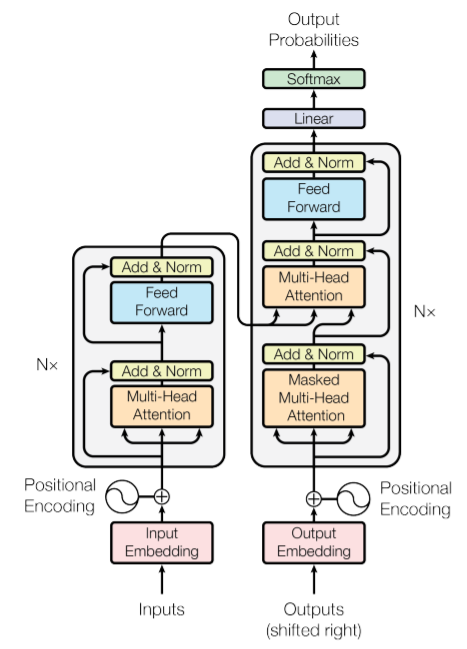
\includegraphics[width=0.50\textwidth]{ai1.png} 
\caption{Transformer 說明示意}
\label{Test}
\end{figure}

在處理過程中大多遇到 Pytorch 套件不相容、版本過舊的問題,這類問題來源大多是  Pytorch 早期開發功能變動所造成,但可以從 HarvardNLP 與 Chatbot using Transformers 的過程中看出整個 Transformer 的設計概念與運作,程式碼的版本進行查錯與修正後執行,而後續兩個範例的 Epoch 等訓練結果,則放於附件 1 與 附件 2 進行呈現。

%\newpage

\section{附件 1}

下為 HarvardNLP 的 The Annotated Transformer 實際測試狀況。

\begin{verbatim}
Epoch Step: 1 Loss: 2.952445 Tokens per Sec: 576.319092
Epoch Step: 1 Loss: 1.998418 Tokens per Sec: 698.345398
tensor(1.9607)
Epoch Step: 1 Loss: 1.944340 Tokens per Sec: 607.740173
Epoch Step: 1 Loss: 1.703401 Tokens per Sec: 697.352722
tensor(1.6663)
Epoch Step: 1 Loss: 1.836476 Tokens per Sec: 608.583740
Epoch Step: 1 Loss: 1.518878 Tokens per Sec: 698.963074
tensor(1.4429)
Epoch Step: 1 Loss: 1.751896 Tokens per Sec: 611.272522
Epoch Step: 1 Loss: 1.445300 Tokens per Sec: 699.340576
tensor(1.4257)
Epoch Step: 1 Loss: 1.457413 Tokens per Sec: 609.735352
Epoch Step: 1 Loss: 0.952619 Tokens per Sec: 700.159241
tensor(0.9635)
Epoch Step: 1 Loss: 1.194762 Tokens per Sec: 603.452271
Epoch Step: 1 Loss: 0.720170 Tokens per Sec: 699.754761
tensor(0.6950)
Epoch Step: 1 Loss: 1.114729 Tokens per Sec: 610.193848
Epoch Step: 1 Loss: 0.482503 Tokens per Sec: 694.832153
tensor(0.4766)
Epoch Step: 1 Loss: 0.910544 Tokens per Sec: 605.345947
Epoch Step: 1 Loss: 0.245647 Tokens per Sec: 699.077209
tensor(0.3241)
Epoch Step: 1 Loss: 0.579662 Tokens per Sec: 606.469055
Epoch Step: 1 Loss: 0.210620 Tokens per Sec: 678.093811
tensor(0.2678)
Epoch Step: 1 Loss: 0.556862 Tokens per Sec: 575.055847
Epoch Step: 1 Loss: 0.189768 Tokens per Sec: 690.105469
tensor(0.2050)
\end{verbatim}

\newpage

\section{附件 2}

fawazsammani/chatbot-transformer 的  Chatbot using Transformers 實際測試狀況。

% 第一段不分栏
% XXXXXXXXXXX

% \columnseprule=1pt         % 实现插入分隔线
\begin{multicols}{2}       % 分两栏 若花括号中为3则是分三列
\begin{verbatim}
Epoch [0][0/2217]	Loss: 8.676
Epoch [0][100/2217]	Loss: 7.872
Epoch [0][200/2217]	Loss: 7.151
Epoch [0][300/2217]	Loss: 6.625
Epoch [0][400/2217]	Loss: 6.282
Epoch [0][500/2217]	Loss: 6.040
Epoch [0][600/2217]	Loss: 5.859
Epoch [0][700/2217]	Loss: 5.713
Epoch [0][800/2217]	Loss: 5.598
Epoch [0][900/2217]	Loss: 5.500
Epoch [0][1000/2217]	Loss: 5.418
Epoch [0][1100/2217]	Loss: 5.348
Epoch [0][1200/2217]	Loss: 5.286
Epoch [0][1300/2217]	Loss: 5.232
Epoch [0][1400/2217]	Loss: 5.186
Epoch [0][1500/2217]	Loss: 5.143
Epoch [0][1600/2217]	Loss: 5.106
Epoch [0][1700/2217]	Loss: 5.073
Epoch [0][1800/2217]	Loss: 5.041
Epoch [0][1900/2217]	Loss: 5.013
Epoch [0][2000/2217]	Loss: 4.987
Epoch [0][2100/2217]	Loss: 4.963
Epoch [0][2200/2217]	Loss: 4.942
Epoch [1][0/2217]	Loss: 4.406
Epoch [1][100/2217]	Loss: 4.406
Epoch [1][200/2217]	Loss: 4.418
Epoch [1][300/2217]	Loss: 4.413
Epoch [1][400/2217]	Loss: 4.416
Epoch [1][500/2217]	Loss: 4.412
Epoch [1][600/2217]	Loss: 4.415
Epoch [1][700/2217]	Loss: 4.414
Epoch [1][800/2217]	Loss: 4.414
Epoch [1][900/2217]	Loss: 4.415
Epoch [1][1000/2217]	Loss: 4.413
Epoch [1][1100/2217]	Loss: 4.413
Epoch [1][1200/2217]	Loss: 4.412
Epoch [1][1300/2217]	Loss: 4.412
Epoch [1][1400/2217]	Loss: 4.410
Epoch [1][1500/2217]	Loss: 4.409
Epoch [1][1600/2217]	Loss: 4.408
Epoch [1][1700/2217]	Loss: 4.407
Epoch [1][1800/2217]	Loss: 4.406
Epoch [1][1900/2217]	Loss: 4.405
Epoch [1][2000/2217]	Loss: 4.404
Epoch [1][2100/2217]	Loss: 4.404
Epoch [1][2200/2217]	Loss: 4.404
Epoch [2][0/2217]	Loss: 4.253
Epoch [2][100/2217]	Loss: 4.307
Epoch [2][200/2217]	Loss: 4.302
Epoch [2][300/2217]	Loss: 4.304
Epoch [2][400/2217]	Loss: 4.304
Epoch [2][500/2217]	Loss: 4.307
Epoch [2][600/2217]	Loss: 4.307
Epoch [2][700/2217]	Loss: 4.309
Epoch [2][800/2217]	Loss: 4.310
Epoch [2][900/2217]	Loss: 4.310
Epoch [2][1000/2217]	Loss: 4.310
Epoch [2][1100/2217]	Loss: 4.310
Epoch [2][1200/2217]	Loss: 4.309
Epoch [2][1300/2217]	Loss: 4.309
Epoch [2][1400/2217]	Loss: 4.308
Epoch [2][1500/2217]	Loss: 4.308
Epoch [2][1600/2217]	Loss: 4.307
Epoch [2][1700/2217]	Loss: 4.306
Epoch [2][1800/2217]	Loss: 4.305
Epoch [2][1900/2217]	Loss: 4.303
Epoch [2][2000/2217]	Loss: 4.303
Epoch [2][2100/2217]	Loss: 4.302
Epoch [2][2200/2217]	Loss: 4.301
Epoch [3][0/2217]	Loss: 4.211
Epoch [3][100/2217]	Loss: 4.194
Epoch [3][200/2217]	Loss: 4.191
Epoch [3][300/2217]	Loss: 4.191
Epoch [3][400/2217]	Loss: 4.193
Epoch [3][500/2217]	Loss: 4.189
Epoch [3][600/2217]	Loss: 4.189
Epoch [3][700/2217]	Loss: 4.189
Epoch [3][800/2217]	Loss: 4.191
Epoch [3][900/2217]	Loss: 4.194
Epoch [3][1000/2217]	Loss: 4.195
Epoch [3][1100/2217]	Loss: 4.197
Epoch [3][1200/2217]	Loss: 4.198
Epoch [3][1300/2217]	Loss: 4.197
Epoch [3][1400/2217]	Loss: 4.199
Epoch [3][1500/2217]	Loss: 4.200
Epoch [3][1600/2217]	Loss: 4.201
Epoch [3][1700/2217]	Loss: 4.202
Epoch [3][1800/2217]	Loss: 4.202
Epoch [3][1900/2217]	Loss: 4.202
Epoch [3][2000/2217]	Loss: 4.202
Epoch [3][2100/2217]	Loss: 4.202
Epoch [3][2200/2217]	Loss: 4.202
Epoch [4][0/2217]	Loss: 4.160
Epoch [4][100/2217]	Loss: 4.089
Epoch [4][200/2217]	Loss: 4.089
Epoch [4][300/2217]	Loss: 4.097
Epoch [4][400/2217]	Loss: 4.102
Epoch [4][500/2217]	Loss: 4.107
Epoch [4][600/2217]	Loss: 4.110
Epoch [4][700/2217]	Loss: 4.113
Epoch [4][800/2217]	Loss: 4.115
Epoch [4][900/2217]	Loss: 4.118
Epoch [4][1000/2217]	Loss: 4.120
Epoch [4][1100/2217]	Loss: 4.121
Epoch [4][1200/2217]	Loss: 4.122
Epoch [4][1300/2217]	Loss: 4.124
Epoch [4][1400/2217]	Loss: 4.125
Epoch [4][1500/2217]	Loss: 4.125
Epoch [4][1600/2217]	Loss: 4.126
Epoch [4][1700/2217]	Loss: 4.126
Epoch [4][1800/2217]	Loss: 4.126
Epoch [4][1900/2217]	Loss: 4.127
Epoch [4][2000/2217]	Loss: 4.128
Epoch [4][2100/2217]	Loss: 4.129
Epoch [4][2200/2217]	Loss: 4.129
Epoch [5][0/2217]	Loss: 4.043
Epoch [5][100/2217]	Loss: 4.040
Epoch [5][200/2217]	Loss: 4.034
Epoch [5][300/2217]	Loss: 4.038
Epoch [5][400/2217]	Loss: 4.041
Epoch [5][500/2217]	Loss: 4.041
Epoch [5][600/2217]	Loss: 4.044
Epoch [5][700/2217]	Loss: 4.047
Epoch [5][800/2217]	Loss: 4.051
Epoch [5][900/2217]	Loss: 4.053
Epoch [5][1000/2217]	Loss: 4.055
Epoch [5][1100/2217]	Loss: 4.056
Epoch [5][1200/2217]	Loss: 4.058
Epoch [5][1300/2217]	Loss: 4.058
Epoch [5][1400/2217]	Loss: 4.060
Epoch [5][1500/2217]	Loss: 4.063
Epoch [5][1600/2217]	Loss: 4.065
Epoch [5][1700/2217]	Loss: 4.067
Epoch [5][1800/2217]	Loss: 4.068
Epoch [5][1900/2217]	Loss: 4.069
Epoch [5][2000/2217]	Loss: 4.070
Epoch [5][2100/2217]	Loss: 4.070
Epoch [5][2200/2217]	Loss: 4.071
Epoch [6][0/2217]	Loss: 4.017
Epoch [6][100/2217]	Loss: 3.981
Epoch [6][200/2217]	Loss: 3.975
Epoch [6][300/2217]	Loss: 3.982
Epoch [6][400/2217]	Loss: 3.987
Epoch [6][500/2217]	Loss: 3.989
Epoch [6][600/2217]	Loss: 3.994
Epoch [6][700/2217]	Loss: 3.997
Epoch [6][800/2217]	Loss: 4.001
Epoch [6][900/2217]	Loss: 4.000
Epoch [6][1000/2217]	Loss: 4.001
Epoch [6][1100/2217]	Loss: 4.004
Epoch [6][1200/2217]	Loss: 4.006
Epoch [6][1300/2217]	Loss: 4.009
Epoch [6][1400/2217]	Loss: 4.011
Epoch [6][1500/2217]	Loss: 4.014
Epoch [6][1600/2217]	Loss: 4.015
Epoch [6][1700/2217]	Loss: 4.017
Epoch [6][1800/2217]	Loss: 4.018
Epoch [6][1900/2217]	Loss: 4.019
Epoch [6][2000/2217]	Loss: 4.020
Epoch [6][2100/2217]	Loss: 4.021
Epoch [6][2200/2217]	Loss: 4.022
Epoch [7][0/2217]	Loss: 3.922
Epoch [7][100/2217]	Loss: 3.929
Epoch [7][200/2217]	Loss: 3.929
Epoch [7][300/2217]	Loss: 3.933
Epoch [7][400/2217]	Loss: 3.936
Epoch [7][500/2217]	Loss: 3.943
Epoch [7][600/2217]	Loss: 3.948
Epoch [7][700/2217]	Loss: 3.950
Epoch [7][800/2217]	Loss: 3.953
Epoch [7][900/2217]	Loss: 3.957
Epoch [7][1000/2217]	Loss: 3.959
Epoch [7][1100/2217]	Loss: 3.962
Epoch [7][1200/2217]	Loss: 3.964
Epoch [7][1300/2217]	Loss: 3.965
Epoch [7][1400/2217]	Loss: 3.966
Epoch [7][1500/2217]	Loss: 3.968
Epoch [7][1600/2217]	Loss: 3.970
Epoch [7][1700/2217]	Loss: 3.972
Epoch [7][1800/2217]	Loss: 3.973
Epoch [7][1900/2217]	Loss: 3.975
Epoch [7][2000/2217]	Loss: 3.977
Epoch [7][2100/2217]	Loss: 3.978
Epoch [7][2200/2217]	Loss: 3.979
Epoch [8][0/2217]	Loss: 4.027
Epoch [8][100/2217]	Loss: 3.880
Epoch [8][200/2217]	Loss: 3.892
Epoch [8][300/2217]	Loss: 3.898
Epoch [8][400/2217]	Loss: 3.900
Epoch [8][500/2217]	Loss: 3.902
Epoch [8][600/2217]	Loss: 3.904
Epoch [8][700/2217]	Loss: 3.909
Epoch [8][800/2217]	Loss: 3.910
Epoch [8][900/2217]	Loss: 3.913
Epoch [8][1000/2217]	Loss: 3.917
Epoch [8][1100/2217]	Loss: 3.920
Epoch [8][1200/2217]	Loss: 3.923
Epoch [8][1300/2217]	Loss: 3.925
Epoch [8][1400/2217]	Loss: 3.928
Epoch [8][1500/2217]	Loss: 3.929
Epoch [8][1600/2217]	Loss: 3.931
Epoch [8][1700/2217]	Loss: 3.931
Epoch [8][1800/2217]	Loss: 3.934
Epoch [8][1900/2217]	Loss: 3.935
Epoch [8][2000/2217]	Loss: 3.937
Epoch [8][2100/2217]	Loss: 3.939
Epoch [8][2200/2217]	Loss: 3.940
Epoch [9][0/2217]	Loss: 3.719
Epoch [9][100/2217]	Loss: 3.839
Epoch [9][200/2217]	Loss: 3.850
Epoch [9][300/2217]	Loss: 3.849
Epoch [9][400/2217]	Loss: 3.854
Epoch [9][500/2217]	Loss: 3.860
Epoch [9][600/2217]	Loss: 3.864
Epoch [9][700/2217]	Loss: 3.868
Epoch [9][800/2217]	Loss: 3.871
Epoch [9][900/2217]	Loss: 3.876
Epoch [9][1000/2217]	Loss: 3.878
Epoch [9][1100/2217]	Loss: 3.882
Epoch [9][1200/2217]	Loss: 3.886
Epoch [9][1300/2217]	Loss: 3.887
Epoch [9][1400/2217]	Loss: 3.889
Epoch [9][1500/2217]	Loss: 3.892
Epoch [9][1600/2217]	Loss: 3.894
Epoch [9][1700/2217]	Loss: 3.896
Epoch [9][1800/2217]	Loss: 3.899
Epoch [9][1900/2217]	Loss: 3.901
Epoch [9][2000/2217]	Loss: 3.903
Epoch [9][2100/2217]	Loss: 3.905
Epoch [9][2200/2217]	Loss: 3.907
\end{verbatim}
\end{multicols}


%\begin{enumerate}
%\item Y
%\item A
%\end{enumerate}

% \newpage

\clearpage

\end{document}